\documentclass[runningheads]{llncs}
\usepackage{amsmath,graphicx,booktabs,url,longtable}
\title{Exact Capacity Allocation Profiles for Vehicle Routing with Tight Fleets}
\titlerunning{Exact Capacity Allocation Profiles for Tight Fleets}
\author{Kha-Anh-Son Vuong\inst{1}\orcidID{0009-0006-3435-7990} \and Luong-Thanh-Tra Ngo\inst{2}\orcidID{0009-0003-2268-3498}}
\authorrunning{Kha-Anh-Son Vuong and Luong-Thanh-Tra Ngo}
\institute{School of Industrial Engineering and Management, Ho Chi Minh City International University, Viet Nam National University Ho Chi Minh City, Vietnam\\
\email{anhson.vuongkha@gmail.com}
\and FPT University, Ho Chi Minh Campus, Vietnam\\
Both authors contributed equally and share first authorship.\\
Corresponding author: Luong-Thanh-Tra Ngo, \email{TraNLT2@fe.edu.vn}}
\begin{document}
\maketitle
\begin{abstract}
When total fleet capacity equals demand, a dispatcher buying four extra units must decide which vehicles receive them. We group customer partitions by sorted route overloads to compute the minimum distance and number of feasible partitions for every allocation. On 55 four-vehicle QOBLIB XSH instances, choosing the allocation after observing demand shortened the optimum relative to equal allocation in 41 cases (median reduction across all cases $1.48\%$, maximum $14.26\%$). In leave-one-out evaluation, every training fold selected three units on one vehicle and one on another. This split attained the optimum on 45 held-out instances. After route pricing, a single profile returned all five design optima and partition counts in a median of 0.058 seconds, compared with 1.452 seconds for five time-limited distance-only MILP solves. On 30 six-vehicle instances with CVRPLIB-X coordinates and generated demands, the adaptive choice improved on the most even allocation in 29 cases but on the three-plus-one split in only 14. An exact join that anchors three customers preserved all class counts and optima and reduced end-to-end computation time by a median factor of 3.59.
\keywords{Capacitated vehicle routing; Fleet capacity allocation; Set partitioning; Exact enumeration}
\end{abstract}

\section{Introduction}
A dispatcher has four identical vehicles, each fully loaded, and can add four units of carrying capacity. On QOBLIB instance XSH-n20-k4-09, giving one unit to each vehicle yields a shortest total distance of 680. Giving three units to one vehicle and one to another brings the distance down to 585. Splitting the units two and two gives the optimum of 583. The vehicles serve the same customers in all three cases. What changes is which customers can share a tour.

This example poses two decisions. A dispatcher who can configure vehicles after observing demand wants the best allocation for that map. A fleet operator who must commit earlier wants a fixed allocation that performs well across maps. To measure the cost of committing early, we compute the optimum for every allocation on each map, then evaluate a fixed allocation selected on other maps.

Our starting point is the tight-capacity routing benchmark~\cite{qob} and its published baseline optima~\cite{tc}. We group partitions of customers by the extra capacity their routes require. Each group records its minimum distance and its number of partitions. A single profile thus answers two questions for any allocation within budget: how short the routes can be and how many ways the customers can be assigned to routes. With six vehicles, restricting which triples of routes can be joined reduces the work. We derive a correction for the number of times each partition appears in those joins, preserving the counts as well as the optima.

\section{Related Work}
Balinski and Quandt~\cite{bq} formulate routing as the selection of feasible routes. Baldacci et al.~\cite{master} strengthen the resulting set-partitioning relaxation with additional cuts. Pessoa et al.~\cite{generic} use branch-cut-and-price to solve a range of routing problems. Our output includes the number of partitions at each overload profile, even when their routes are expensive. We therefore price every eligible customer set using Held--Karp dynamic programming~\cite{hk}. This difference in outputs matters when comparing runtimes.

Muñoz-Herrera and Suchan~\cite{landscape} relate vehicle utilization to search trajectories under different neighborhood operators. Dollevoet and Spliet~\cite{pre} use subset sums to tighten capacity while preserving feasible solutions. Here we vary capacity and measure how many partitions become feasible and how much distance they save.

Golden et al.~\cite{fleet} optimize fleet composition under fixed and variable costs. We keep the fleet size fixed and compute distance as a function of upgrade count. This curve reveals efficient choices that a uniform upgrade fee can miss~\cite{pareto}.

Aggoune-Mtalaa et al.~\cite{modules} study how to allocate modules in urban freight routing. We assume a single divisible integer payload resource, fungible increments and known demand at dispatch. Holding the total increment fixed allows us to measure the distance penalty of a fixed allocation in isolation. Our model omits coupling, energy and module-handling costs.

We use the X benchmark~\cite{x} in three ways: 20-customer samples retain their original demands, six-vehicle samples retain only the parent geometry, and full parents supply demands for a load-count diagnostic. Only the samples undergo route optimization.

The TC-Exact technical note~\cite{tc} reports optimal costs at the original tight capacities. We reproduce those values before varying capacity. Joining complementary subsets is related to methods that count disjoint set packings by combining partial packings~\cite{pack} and to subset convolution~\cite{convolve}. Here each partial packing carries routing costs and overloads. The counting correction depends on how many routes contain the distinguished customers.

\section{Quantities That Capacity Can Change}
Let $N$ be a set of $n$ customers, each with positive integer demand $d_i$. A fixed fleet of $k$ vehicles serves them from one depot. Each vehicle makes one nonempty tour and has integer capacity $C$. Define $D=\sum_{i\in N}d_i$, the fleet slack $\Delta=kC-D$, and $d(S)=\sum_{i\in S}d_i$. A feasible partition $P$ is an unordered collection of $k$ disjoint nonempty subsets whose union is $N$ and whose individual loads are at most $C$. Write $\mathcal P(C)$ for the family of such partitions and $H(C)=|\mathcal P(C)|$ for its cardinality. Let $t(S)$ denote the minimum cost of a closed depot tour through $S$. The optimal distance is
\begin{equation}
 z(C)=\min_{P\in\mathcal P(C)}\ \sum_{S\in P}t(S).
\end{equation}
This definition counts a partition once even if several visit orders attain the same cost. Integer edge lengths are the nearest integers to Euclidean distances, obtained as $\lfloor d+0.5\rfloor$ before summing the edges.

\paragraph{The interval of admissible loads.}
If one vehicle serves $S$, the other $k-1$ vehicles must carry $D-d(S)$ units. It follows that every member of every feasible partition satisfies
\begin{equation}\label{eq:filter}
 L(C)=\max\{1,D-(k-1)C\}=\max\{1,C-\Delta\}
 \ \leq d(S)\leq C .
\end{equation}
At $\Delta=0$ every vehicle carries exactly $C$. Raising the capacity of a tight four-vehicle fleet from $Q$ to $Q+1$ allows loads from $\max\{1,Q-3\}$ to $Q+1$. A set in this interval is usable only if its complement fits in the remaining vehicles.

We compute the retained fraction $r(C)$ by counting subset loads between $L(C)$ and $C$ and dividing by the number of nonempty subsets with load at most $C$. The supplement gives the generating function and recurrence.

\paragraph{A control for spatial assignment.}
Permuting the demands over fixed customer locations induces a bijection on subsets and on feasible partitions. The bijection preserves loads and therefore $H(C)$ at every capacity. It need not preserve $t(S)$ because the points on the mapped tour can differ. The relative optimal-distance change
\begin{equation}\label{eq:drop}
 b_i=100\,[z_i(Q_i)-z_i(Q_i+1)]/z_i(Q_i)
\end{equation}
can thus vary while the combinatorial expansion $H_i(Q_i+1)/H_i(Q_i)$ is held exactly fixed. This paired control retains the depot, the multiset of locations, the entire distance matrix and the demand histogram. It tests the role of matching a demand to a point; it does not generate a new spatial point process.

\section{Exact Computation and Verification}
Figure~\ref{fig:pipeline} traces a route from pricing to the allocation decision. Both fleet sizes use the same overload profile as their output.
\begin{figure}[tb]\centering
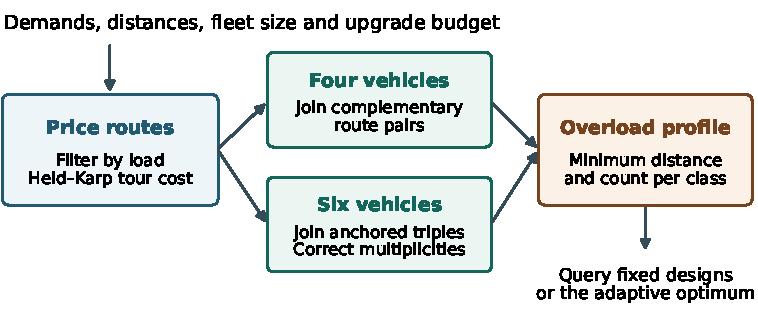
\includegraphics[width=\linewidth]{allocation-pipeline.pdf}
\caption{Computing one profile for all allocations of a fixed budget. Each branch combines disjoint routes that together cover every customer. Counts and costs are retained by sorted overload class.}\label{fig:pipeline}
\end{figure}
\paragraph{Pricing a customer set.}
We enumerate customer sets recursively, pruning a branch when its load exceeds capacity or its remaining demand cannot bring it to the lower bound. Held--Karp dynamic programming~\cite{hk} then computes the shortest closed depot tour for each surviving set $S$ in $O(|S|^2 2^{|S|})$ time. Thus sets of different sizes can have substantially different pricing costs.

\paragraph{Choosing four routes.}
Each priced set has a bit mask. Choosing the route that contains the smallest uncovered customer at each step orders each partition uniquely. After two choices, we cache the number of ways to split the remainder, the minimum summed cost, its multiplicity and the next distinct cost, if one exists.

For upgrades of a fixed size, the same search labels each route by whether it exceeds base capacity. For each remaining mask and route count, we retain a minimum cost and count at each exact number of upgrades. Prefix minima give the optimum under each upgrade budget. The supplement gives the recurrence and the four-vehicle cache construction.

\paragraph{One profile for all capacity allocations.}
Suppose that vehicle $i$ can receive $a_i$ extra units and that $\sum_i a_i=B$. For a partition $P$ define the overload of route $S$ by $e(S)=(d(S)-Q)_+$. Its minimum total upgrade requirement is $E(P)=\sum_{S\in P}e(S)$. Necessity follows by summing route overloads; sufficiency follows by giving each route exactly its overload and assigning any surplus arbitrarily. When the fleet starts tight, $\sum_S(d(S)-Q)=0$, so
\[
 E(P)=\tfrac12\sum_{S\in P}|d(S)-Q|.
\]
Any partition achievable with $B$ units has every load in $[Q-B,Q+B]$. The lower endpoint follows because total underload equals total overload. For a fixed allocation, sort both its increments and the overloads in ascending order. A feasible assignment exists exactly when each ordered overload is no larger than the corresponding increment. Matching in order proves sufficiency. If a component exceeds its allowance, too many large overloads compete for too few large increments.

For four vehicles, we first group disjoint route pairs by their customer union and the two sorted overloads. Each group stores a count, the least summed tour cost and a witness. Joining complementary customer unions gives the full sorted overload tuple and an optimal witness for that tuple. The costs add and the counts multiply because the two pairs serve disjoint customers. We orient the join using the side containing the first customer. A four-route partition then occurs once for each of its three unordered pairings, so we divide its accumulated class count by three. Componentwise filtering of the resulting tuples answers every fixed-allocation query; taking the minimum over all tuples gives the best allocation for the known instance. Counts are retained by exact tuple to avoid double-counting partitions compatible with several designs.

\paragraph{Restricting the six-route join using anchor customers.}
The unrestricted six-route join forms all complementary triples. Choose $1\leq a\leq3$ distinguished customers and retain only triple masks that contain all or none of them. Orient the join with all distinguished customers on the left. If the anchors occupy $s$ distinct routes of a particular six-route partition, those $s$ routes must be on the left. Any $3-s$ of the remaining $6-s$ routes can complete that side, so the partition appears $m_s=\binom{6-s}{3-s}$ times. For $s=1,2,3$ these multiplicities are 10, 4 and 1. A compatible split exists for every partition. Consequently the minimum cost and a minimizing witness survive this restriction.

Figure~\ref{fig:anchor-example} illustrates the case $s=2$.
\begin{figure}[tb]\centering
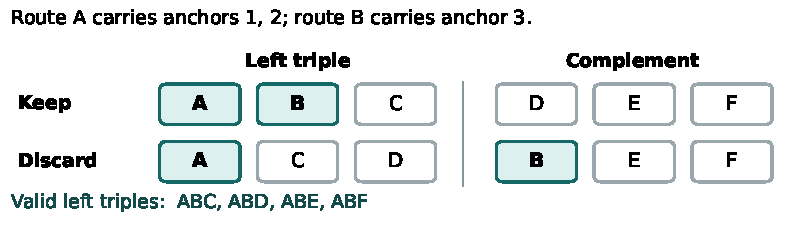
\includegraphics[width=\linewidth]{anchor-example.pdf}
\caption{One six-route partition with three anchors on two routes. Keeping all anchors on the left permits four choices of the third route. Each valid split contributes one quarter of this partition's count.}\label{fig:anchor-example}
\end{figure}
Counts require a correction before aggregating partitions with the same overloads: attach the indicator of meeting an anchor to each route and sum it within partial groups. Multiply each oriented join count by $20/m_s$, accumulate by overload tuple, and divide the result by 20. Each partition now contributes exactly one. For a $2h$-route fleet the same reasoning gives $\binom{2h-s}{h-s}$ whenever $1\leq a\leq h$. We implement and benchmark the six-route case. The $a$ anchor bits in a retained triple mask share a single value, so its direct index uses $2^{n-a+1}$ heads. This bound concerns the triple index; pair storage and the number of profile entries also affect total memory.
\paragraph{Early and late filtering.}
Early filtering applies $L(C)$ before tour pricing. Late filtering prices all nonempty sets with load at most $C$ and applies the same bound during cover search. Equation~(\ref{eq:filter}) guarantees that the two modes agree on partition count, optimal cost, optimal multiplicity and next distinct cost.

\paragraph{What each check establishes.}
We replay the public TC-Exact program on all 55 original instances and compare the objective with the input header. We also solve a binary set-partitioning master with one variable $y_S$ per priced candidate:
\begin{equation}
 \min\sum_S t(S)y_S,\quad \sum_{S\ni i}y_S=1\ (i\in N),\quad
 \sum_S y_S=4,\quad y_S\in\{0,1\}.
\end{equation}
The master checks route selection using independently implemented optimization and shared prices. For all capacity settings a Python dynamic program reconstructs tours for the winning sets. The official QOBLIB Rust checker examines the exported routes at the tested capacity; we additionally compare its computed cost with the reported objective. A successful route check establishes feasibility and achieved cost. Exhaustive pricing and coverage establish optimality in our implementation.

An independent edge model checks selected positive-slack cases directly from distances and demands. Rounded-capacity cuts supply valid lower bounds at the time limit. The supplement gives the formulation.
\section{Experimental Design}
\paragraph{Capacity sweep.}
All 55 QOBLIB XSH-n20-k4 instances have 20 customers, four vehicles and $D=4Q$. We solve each at its original capacity and after increasing per-vehicle capacity by $1$, $\lceil0.02Q\rceil$, $\lceil0.05Q\rceil$ and $\lceil0.10Q\rceil$. The feasible sets are nested, so the partition count cannot fall and the optimum cannot rise.

\paragraph{Pairing and timing.}
We record candidate and partition counts, minimum cost, its multiplicity and the next distinct cost. We compute ratios within instances before taking medians. Base timings use five repetitions and modified capacities use two. The early/late comparison uses three repetitions per mode at three slack levels, alternating mode order across cases and dividing median late time by median early time. Timings include pricing and cover search. We used an Apple M1, Apple Clang 21 (C++17, -O3), Python 3.11 and SciPy 1.12.

\paragraph{Demand reassignment.}
We draw 51 deterministic pseudorandom shuffles for each original XSH demand vector. Seeds are $20261121+100i+j$, with $i=0,\ldots,54$ in input-name order and $j=0,\ldots,50$. For each shuffle we solve at $Q$ and $Q+1$, compare both partition and candidate counts against the unshuffled inputs, and reconstruct the two sets of optimal tours. We summarize the 51 percentage reductions by their median for each instance before comparing with the original assignment. The 2,805 shuffles share 55 base instances. We first ran five assignments per input and then fixed the expanded sample size at 51. We report the initial and additional batches separately as a sensitivity check.

Two disjoint 20-customer samples per external parent test filtering on other demand distributions. On the ten full parents we compute only the subset-load counts. The supplement gives the selection, packing and timing protocols.
\section{Results}
\subsection{The first unit changes which customers can travel together}
All 55 base optima matched TC-Exact and the route master. Every tested increase shortened the optimum on every instance. At one extra unit per vehicle, feasible partitions grew by a median factor of 39.90 (range 16.00--108.32). Distance savings ranged from 3.53\% to 24.14\% (interquartile range 8.00--16.31\%). Table~\ref{tab:sweep} reports medians of within-instance changes.

Figure~\ref{fig:routes} illustrates the capacity change on XSH-n20-k4-01. Giving each vehicle one extra unit increases the number of feasible customer partitions from 2,520 to 97,951 and reduces the optimal distance from 646 to 580.

\begin{figure}[tb]
\centering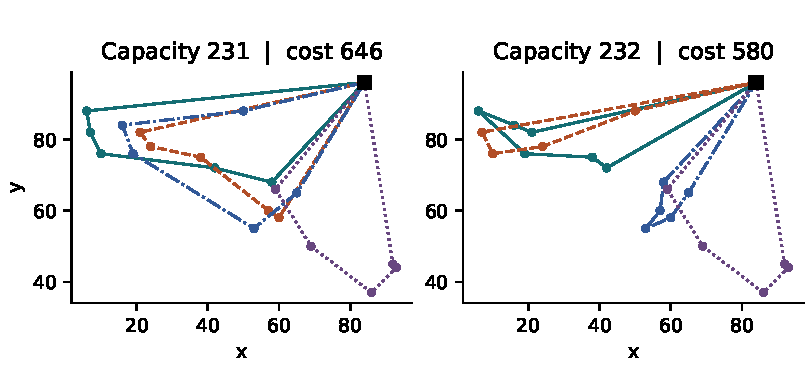
\includegraphics[width=.94\linewidth]{route-example.pdf}
\caption{Optimal tours for XSH-n20-k4-01 at the original capacity and after adding one unit per vehicle. The black square marks the common depot. Line styles distinguish the four routes within each panel. Both panels use the original coordinates and the same scale.}\label{fig:routes}
\end{figure}

\begin{table}[tb]\centering
\caption{Capacity sweep across the 55 XSH instances. Columns report medians. Growth and distance savings are calculated relative to the same instance at $Q$. Times cover pricing and cover search.}\label{tab:sweep}
\begin{tabular}{lrrrrr}\toprule
Increase & Priced sets & Partitions & Paired growth & Saving (\%) & Time (ms)\\\midrule
Base &536&2,334&1.00&0.00&1.74\\
1 unit &2,624&88,338&39.90&10.79&9.40\\
2\% &10,783&5,237,545&2,147&15.64&66.43\\
5\% &22,557&63,376,232&25,045&16.96&175.62\\
10\% &38,279&427,619,367&173,404&18.92&417.97\\\bottomrule
\end{tabular}
\end{table}

On instance 01, raising extra capacity from 2\% to 5\% increased the partition count from 5,601,030 to 64,760,163 while the optimum remained 551. At the next tested capacity the optimum fell to 542.

The supplement plots the between-instance dispersion at each capacity level.


\subsection{Equal spending, different allocations}
Four integer units can be distributed among four interchangeable vehicles in five ways. Table~\ref{tab:allocation} compares all five on the 55 XSH demand maps. The equal allocation reproduces the previous $Q+1$ objective and partition count on every instance. The all-zero overload class also reproduces both base quantities. We independently reconstructed a minimum-cost tour for each route of every retained tuple witness and checked its overloads.

\begin{table}[tb]\centering
\caption{Allocation of the same four extra units on XSH. Tied designs each receive credit. Distance excess is relative to the best allocation on the same instance.}\label{tab:allocation}
\begin{tabular}{lrr}\toprule
Extra units per vehicle & Attains best distance & Median distance excess\\\midrule
$(4,0,0,0)$ & 20/55 & 0.63\%\\
$(3,1,0,0)$ & 45/55 & 0.00\%\\
$(2,2,0,0)$ & 29/55 & 0.00\%\\
$(2,1,1,0)$ & 29/55 & 0.00\%\\
$(1,1,1,1)$ & 14/55 & 1.50\%\\\bottomrule
\end{tabular}
\end{table}

Choosing the allocation after observing the demand map improved on equal allocation in 41 of 55 cases. Relative to the equal-allocation distance, the median reduction was 1.48\% and the largest was 14.26\%. Instance 09, which opens the paper, attained this maximum. Two other designs on that map had the same optimum of 585: $(3,1,0,0)$ admitted 720,424 feasible partitions and $(2,1,1,0)$ admitted 431,249. These counts include partitions of every cost. They distinguish allocations with equal best distance without implying that the additional partitions are equally cheap.

Could a planner obtain most of the benefit from one reusable design? For each held-out XSH instance we selected the allocation with the smallest mean cost relative to equal allocation on the other 54. Every fold selected $(3,1,0,0)$. It tied the instance-specific optimum in 45 cases. The adaptive choice yielded shorter routes in the remaining ten, with a median reduction across all instances of zero, a mean of 0.18\% and a maximum of 3.01\%. Thus much of the apparent gain over equal distribution was available to a simple fixed policy in this suite. The adaptive optimum assumes that capacity can be configured after demands are observed.

\paragraph{Independent route selection.}
As a check on the pair join, a set-partitioning MILP uses one binary variable per priced route and adds $\sum_S e(S)y_S\leq4$ to the coverage and fleet-size equalities. It shares the tour prices, but neither the pair summaries nor the load-tuple enumeration. With ten seconds per instance, the MILP proved the same optimum on 52 of 55 cases. On instances 09, 13 and 28 it timed out with lower bounds and feasible incumbents. We attribute those three optimality results to exact enumeration.

\paragraph{One profile or five fixed-design solves?}
We compared the time to return all five design optima on every XSH instance (Fig.~\ref{fig:five-solves}). Both methods started with the same priced routes and overloads. The profile time includes serializing routes, starting the C++ join, and querying all five designs. The five single-threaded MILP solves shared a coverage matrix. For each design we removed routes exceeding its largest increment and, for each threshold $t=1,\ldots,4$, capped the number of routes with overload at least $t$ at the number of vehicles receiving at least $t$ units. We ran each method once per instance, alternating their order, with a two-second solver limit per design.

\begin{figure}[tb]\centering
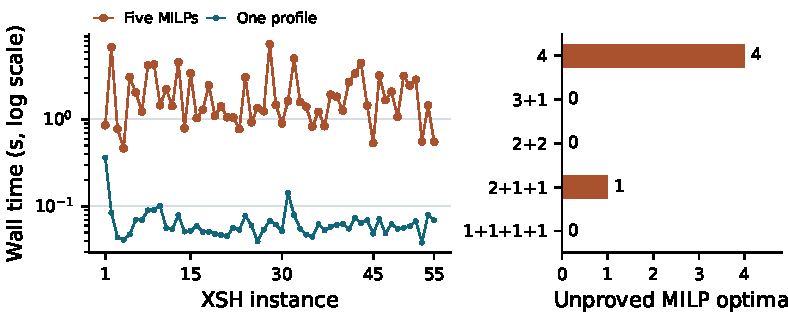
\includegraphics[width=\linewidth]{five-design-benchmark.pdf}
\caption{Five fixed allocations on each of 55 XSH instances. Left: observed time for all five queries after shared pricing, including time-limited solves. Right: number of unproved MILP optima per allocation (two seconds per solve). The profile established all 275 optima and counted the feasible partitions.}\label{fig:five-solves}
\end{figure}

Median times were 0.058 s for the profile and 1.452 s for five MILPs. The profile reproduced all archived optima and counts. The MILPs proved 270 of 275 optima, completing all five on 50 of 55 instances. Each MILP that reported optimality agreed with the profile. The median within-instance ratio of elapsed MILP time to profile time was 26.07$\times$. This ratio describes the two implementations under the stated time limit. The MILPs returned distance bounds and incumbents, while the profile also counted partitions for every design.

\paragraph{Transfer to six vehicles.}
We froze the three-plus-one rule from XSH and tested it first on ten 24-customer instances with six vehicles of base capacity 100, then on twenty further instances. Each uses the depot and 24 sampled customer coordinates of a different X parent. The first ten are the smallest parents in the source repository. Before the extension we sorted the remaining 87 parents by node count and picked 20 evenly spaced ranks, including both endpoints. With seed $20261123+i$ for consecutive sample index $i=0,\ldots,29$, we sampled sites without replacement, then generated six four-customer demand groups. Three integers per group were drawn uniformly from 16 through 34; the fourth filled the group load to 100. We rejected groups whose fourth value was outside that range, then shuffled the 24 demands across the sites. This guarantees a feasible tight base fleet. The parent instances retain their source identities only through their coordinates; demands and capacities are generated for this test. The most even split of four indivisible units is $(1,1,1,1,0,0)$.

A separate Python route pricer enumerates customer sets with load 96--104 and solves their tours by dynamic programming. For a fixed allocation, the route master limits the number of selected routes with excess at least $t$ to the number of vehicles receiving at least $t$ units, for $t=1,\ldots,4$. These four inequalities are equivalent to the sorted matching test. For adaptive allocation the master instead limits summed excess to four. Every returned incumbent was checked for coverage and loads, and its tour costs were verified by visit-order enumeration. The direct adaptive MILP closed six cases in ten seconds each. For the four timeouts we also solved the remaining fixed allocations, budgeting ten seconds per additional design. The five fixed-design feasible sets exhaust the adaptive feasible set. Combining their bounds and incumbents certified all four remaining optima.

On the ten initial geometries, the adaptive allocation beat the even split in all ten cases and the three-plus-one split in six. On the 20 additional geometries, the corresponding counts were 19 and eight. The supplement reports distances for every parent.

The profile join matched all ten initial adaptive MILP certificates and all 32 certified fixed-design costs. On four extension parents, all 12 additional MILP costs agreed. An independent enumeration of $35^3$ covers checked both counts and costs. Across all 30 parents, every join variant returned the same class counts and minima, and reconstructed routes attained those minima. Figure~\ref{fig:anchors} shows how the end-to-end speedups vary across parents. The three-anchor join itself was $3.69\times$ faster at the median (interquartile range $3.44$--$3.87$). The baseline stored 4.53 times as many distinct triple masks at the median.

\begin{figure}[tb]\centering
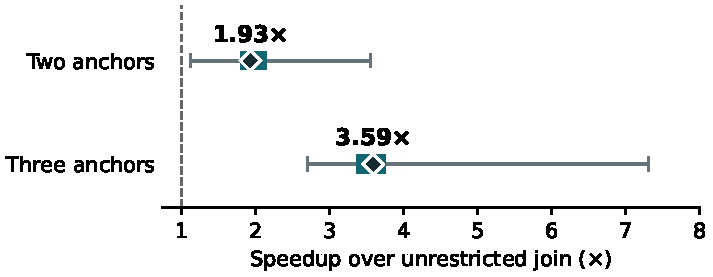
\includegraphics[width=\linewidth]{anchor-speedup.pdf}
\caption{Left: end-to-end speedup including pricing, across 30 geometries. Diamonds mark median baseline-to-variant time ratios, thick bars show the middle 50\%, and thin bars span the observed range. The dashed line marks equal time. We varied mode order and took median times within each parent (three runs per mode on six parents, one on the remaining 24). Right: median number of distinct triple masks stored by each join, in thousands.}\label{fig:anchors}
\end{figure}

\paragraph{Replication under generated demand.}
We crossed ten source geometries with ten shared demand seeds at 24 customers and six vehicles. Each seed builds six four-customer groups of load 100 by redistributing demand within each group. On all 100 combinations the three joins agreed on every class count and minimum cost. Table~\ref{tab:repeat-anchor} reports elapsed time and memory separately from the original 30-parent experiment.

\begin{table}[tb]\centering
\caption{Six-route join replication. Each entry is the median of 100 within-case ratios (unrestricted divided by variant). Wall time includes starting the worker. Memory is sampled peak resident memory across the worker and its children.}\label{tab:repeat-anchor}
\begin{tabular}{lrr}\toprule
Join variant & Wall-time speedup & Peak memory ratio\\\midrule
Two anchors & $1.89\times$ & $1.15\times$\\
Three anchors & $3.13\times$ & $1.73\times$\\\bottomrule
\end{tabular}
\end{table}

\paragraph{When does choosing the allocation pay?}
Figure~\ref{fig:policygain} shows the fraction of instances on which adaptation saves more than a given fraction of the fixed design's distance. At zero the curves count strict improvements. On the six-vehicle set, the even split leaves room to improve on 29 of 30 cases, compared with 14 for three-plus-one. At higher thresholds the curves identify how often those improvements are large enough to matter to a planner.

\begin{figure}[tb]\centering
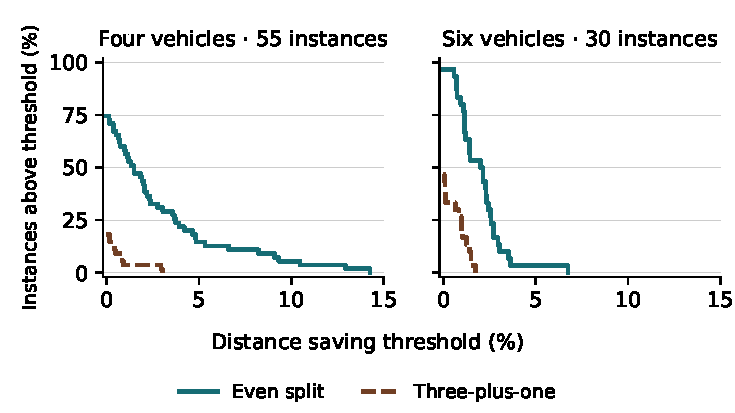
\includegraphics[width=\linewidth]{policy-gain.pdf}
\caption{Distance saved by choosing an allocation after observing demand. Each step gives the percentage of instances with savings strictly above the threshold, relative to the indicated fixed design. Panels use identical scales.}\label{fig:policygain}
\end{figure}

\paragraph{Certifying the value of further optimization.}
Given a feasible three-plus-one plan of distance $U$, a lower bound $L$ on the adaptive optimum bounds its remaining saving by $100(U-L)/U$ percent. We relaxed integrality in the adaptive route master and added up to two rounds of the twelve most violated three-customer subset-row inequalities~\cite{cuts}. For a triple of customers, at most one selected route can serve at least two members. We examined every customer triple after each LP solve. To obtain a valid integer bound we rounded the dual multipliers onto a grid of $10^{-6}$, enforced the signs of inequality multipliers, and reduced the fleet-equality multiplier by the maximum positive dual constraint violation. Every route has fleet coefficient one. We checked every repaired column inequality in integer arithmetic and rounded the resulting lower bound up to the next integer when fractional.

Table~\ref{tab:cert} compares the bounds for the optimal three-plus-one plan supplied as an incumbent. Finding that incumbent is a separate computation. At a 1\% tolerance, cuts certify 19 of the 24 genuinely qualifying cases.
\begin{table}[tb]\centering
\caption{Number of six-vehicle instances (out of 30) where the remaining distance saving is at most the stated tolerance. The last column uses the exact adaptive optimum.}\label{tab:cert}
\begin{tabular}{rrrr}\toprule
Tolerance & Plain LP & LP with cuts & Exact profile\\\midrule
0\% & 1 & 4 & 16\\
0.5\% & 2 & 10 & 20\\
1\% & 3 & 19 & 24\\
2\% & 12 & 29 & 30\\\bottomrule
\end{tabular}
\end{table}
\subsection{How many vehicles need the extra unit?}
Suppose that at most $b$ of the four vehicles can carry $Q+1$, with the rest limited to $Q$. For any partition feasible at $Q+1$, let $u(P)$ count its routes whose load exceeds $Q$. The partition is feasible with budget $b$ exactly when $u(P)\leq b$: assign one upgraded vehicle to each of those routes. We compute $z_b$, the minimum distance under that budget, by classifying every partition by $u(P)$ and taking a cumulative minimum. A separate enumeration reuses the priced sets, reconstructs a witness for every nonempty class and recovers both endpoint optima and both partition counts on all 55 instances.

Because $D=4Q$, four routes simultaneously above $Q$ would exceed total demand. Consequently $z_3=z_4$ in every case. How closely $z_1$ or $z_2$ approaches $z_4$ depends on the data. Table~\ref{tab:upgrades} measures the fraction $(z_0-z_b)/(z_0-z_4)$ within each instance. All 55 denominators are positive.

\begin{table}[tb]\centering
\caption{Partial fleet upgrades on XSH. Savings are relative to those achievable by upgrading all four vehicles. The last column counts instances attaining that optimum.}\label{tab:upgrades}
\begin{tabular}{lrrr}\toprule
Upgraded vehicles & Median partitions & Median saving recovered & Full saving\\\midrule
0 & 2,334 & 0\% & 0/55\\
1 & 32,765 & 94.29\% & 19/55\\
2 & 78,332 & 100\% & 50/55\\
3 or 4 & 88,338 & 100\% & 55/55\\\bottomrule
\end{tabular}
\end{table}

One upgrade shortened every optimum, recovering 4.20--100\% of the available saving (interquartile range 80.77--100\%). On instance 11 the distance fell from 914 to 908 with one upgrade and to 771 with two. A small first gain can therefore conceal a large second gain.

Caching accelerated the full curve computation in all 110 instance--upgrade combinations. At upgrade sizes one and two, the median speedups relative to enumeration were 2.42 and 4.02. A uniform upgrade fee missed four of 150 efficient points at size one and three of 155 at size two. The supplement gives timings and the fee inequalities.
\subsection{Demand placement changes the return on an extra unit}
All 5,610 solves in the shuffle experiment reproduced the original partition and candidate counts at their respective capacities. Of the 2,805 shuffled pairs, 2,721 achieved a strictly shorter optimal distance and 84 had equal optimal distances. The largest observed reduction was 26.36\%. The typical effect, however, was appreciably smaller than on the released assignments (Fig.~\ref{fig:shuffle}). The median across the 55 within-instance medians was 5.70\%, with an interquartile range of 4.46--7.73\%. For each instance we also subtracted its original reduction from its shuffle median. This paired difference had median $-5.08$ percentage points and interquartile range $[-10.10,-2.95]$. Only three instances had a larger shuffle median than the original reduction. The first five draws gave a median instance response of 6.17\%; the additional 46 gave 5.72\%. On nine instances the original gain exceeded every one of the 51 shuffled gains.

\begin{figure}[tb]\centering
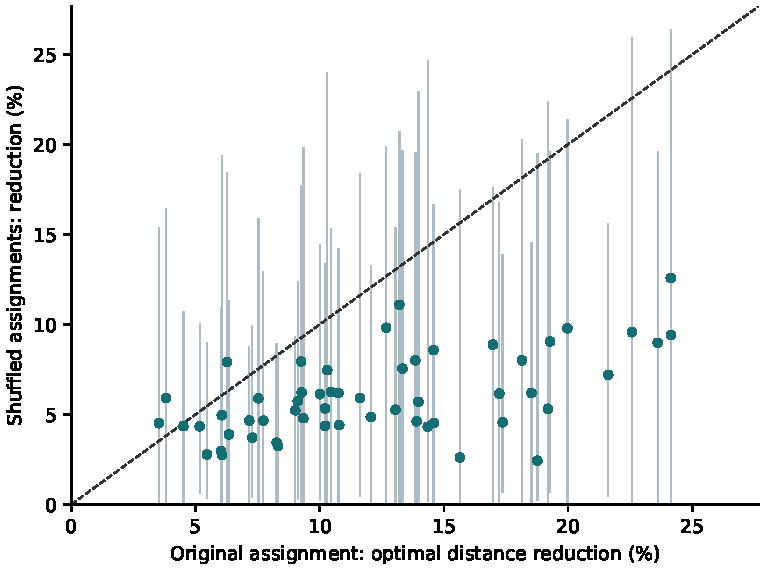
\includegraphics[width=.91\linewidth]{assignment-control.pdf}
\caption{Distance response to one extra unit per vehicle. Each dot represents one base instance; its ordinate is the median over 51 shuffled assignments. Vertical segments span the 51 observed reductions. Points below the identity line gained more from the capacity change under the original placement of demands.}\label{fig:shuffle}
\end{figure}



Each vertical segment in Fig.~\ref{fig:shuffle} holds both partition counts fixed. Across instances, the median difference between the original optimum and the median shuffled optimum was $+14$ distance units at $Q$ and $-23$ at $Q+1$. The spread within each segment measures how much the distance benefit can change solely through reassignment of demands within the observed geometry.

\paragraph{Scope of the load filter and shuffle controls.}
At one extra unit, screening loads before tour pricing improved total time by a median factor of 4.45 on XSH; at 5\% extra capacity the factor fell to 1.04. On external 20-customer samples the one-unit factor was 1.055 among the 18 completed pairs. The median effect of demand reassignment on distance reduction was zero on the nine complete external parents. The supplement reports all exclusions, timing distributions and demand-only profiles.
\subsection{Independent checks at positive slack}
The official checker verified all 275 solutions in the unshuffled sweep. At the 5\% capacity level, we also ran the independent edge formulation on nine instances spaced evenly by rank of one-unit partition growth. Within ten seconds it proved optimality on two and returned lower bounds on the other seven. The supplement lists the nine gaps.



\section{Discussion and Scope}
On a tight fleet, each new feasible grouping has a spatial cost. The reassignment experiment shows that two instances can agree in customer count, fleet size and feasible partition count yet offer different savings from the same upgrade.

For a new fleet, the demand histogram gives a cheap first estimate of filtering selectivity. Both the fraction and absolute number of retained sets matter: even a selective interval can leave billions of tours to price. Distances and route sizes determine the remaining work.

The routing results apply to small tight fleets. The six-vehicle cases use generated demands, and the full X parents contribute only load counts. Distance savings exclude the purchase and operating costs of upgrades. Times come from a single machine, and the 51 shuffles per instance sample only a fraction of demand placements. Comparisons with other exact solvers would also have to account for the cost of returning class counts as well as an optimal route plan.

\section{Conclusion}
The three-plus-one split chosen on other XSH demand maps attained the adaptive optimum on 45 of 55 held-out instances. The same rule remained competitive on the six-vehicle transfer set, where adaptation improved it in 14 of 30 cases. Exact overload profiles identify the exceptions and quantify their cost. Anchoring three customers made these profiles cheaper to compute while preserving every class count and minimum. Transfer to larger fleets remains an open computational question.

\paragraph{Use of AI tools.}
OpenAI Codex assisted with experimental implementation, data analysis, figure generation and manuscript drafting. Statistics were computed from the archived experiment outputs.

\begin{thebibliography}{99}
\bibitem{master} Baldacci, R., Christofides, N., Mingozzi, A.: An exact algorithm for the vehicle routing problem based on the set partitioning formulation with additional cuts. Mathematical Programming \textbf{115}, 351--385 (2008). \doi{10.1007/s10107-007-0178-5}
\bibitem{generic} Pessoa, A., Sadykov, R., Uchoa, E., Vanderbeck, F.: A generic exact solver for vehicle routing and related problems. Mathematical Programming \textbf{183}, 483--523 (2020). \doi{10.1007/s10107-020-01523-z}
\bibitem{pack} Björklund, A., Husfeldt, T., Kaski, P., Koivisto, M.: Counting paths and packings in halves. In: ESA, LNCS, vol. 5757, pp. 578--586 (2009). \url{https://arxiv.org/abs/0904.3093}
\bibitem{convolve} Björklund, A., Husfeldt, T., Kaski, P., Koivisto, M.: Fourier meets Möbius: fast subset convolution. In: ACM STOC, pp. 67--74 (2007). \url{https://arxiv.org/abs/cs/0611101}
\bibitem{modules} Aggoune-Mtalaa, W., Habbas, Z., Ait Ouahmed, A., Khadraoui, D.: Solving new urban freight distribution problems involving modular electric vehicles. IET Intelligent Transport Systems (2015). \doi{10.1049/iet-its.2014.0212}
\bibitem{bq} Balinski, M.L., Quandt, R.E.: On an integer program for a delivery problem. Operations Research \textbf{12}, 300--304 (1964). \doi{10.1287/opre.12.2.300}
\bibitem{pareto} Przybylski, A., Gandibleux, X., Ehrgott, M.: Two phase algorithms for the bi-objective assignment problem. European Journal of Operational Research (2008). \url{https://www.sciencedirect.com/science/article/pii/S0377221707000781}
\bibitem{pre} Dollevoet, T., Spliet, R.: Preprocessing to reduce vehicle capacity for routing problems. Operations Research Forum \textbf{4}, 42 (2023). \doi{10.1007/s43069-023-00220-9}
\bibitem{fleet} Golden, B., Assad, A., Levy, L., Gheysens, F.: The fleet size and mix vehicle routing problem. Computers \& Operations Research \textbf{11}, 49--66 (1984). \doi{10.1016/0305-0548(84)90007-8}
\bibitem{cuts} Jepsen, M., Petersen, B., Spoorendonk, S., Pisinger, D.: Subset-row inequalities applied to the vehicle-routing problem with time windows. Operations Research \textbf{56}, 497--511 (2008). \doi{10.1287/opre.1070.0449}
\bibitem{hk} Held, M., Karp, R.M.: A dynamic programming approach to sequencing problems. Journal of the Society for Industrial and Applied Mathematics \textbf{10}, 196--210 (1962). \doi{10.1137/0110015}
\bibitem{landscape} Muñoz-Herrera, S., Suchan, K.: Constrained fitness landscape analysis of capacitated vehicle routing problems. Entropy \textbf{24}, 53 (2022). \doi{10.3390/e24010053}
\bibitem{qob} Koch, T., Bernal Neira, D.E., Chen, Y., et al.: The Quantum Optimization Benchmarking Library. Nature Computational Science \textbf{6}, 653--671 (2026). \doi{10.1038/s43588-026-00991-1}
\bibitem{x} Uchoa, E., Pecin, D., Pessoa, A., Poggi, M., Subramanian, A., Vidal, T.: New benchmark instances for the capacitated vehicle routing problem. European Journal of Operational Research \textbf{257}, 845--858 (2017). \doi{10.1016/j.ejor.2016.08.012}
\bibitem{tc} Vuong Kha Anh Son: Closing the QOBLIB CVRP benchmark: Exact optimality certificates and subspace simulated quantum annealing for tight-capacity routing. Public technical note (2026), revision 675fbfc. \url{https://github.com/vkas0812-sys/qoblib-routing-exact-sqa}
\end{thebibliography}

\end{document}
